%Probleme:
  %Umgebungsruck p0?
  %Kursive Buchstaben in Formel
  %Referenzen werfen Fehler

\section{Auswertung}
\label{sec:auswertung}
\subsection{Messdaten}
In den folgenden Tabellen sind die während des Experimentes aufgenommenen Daten aufgeführt:
\begin{table}[H]
  \centering
      \caption{Messwerte der Temperatur im Druckbereich über $\SI{1}{bar}$}
      \label{tab:hohe}
      \sisetup{table-format=6.2}
      \begin{tabular}{S S}
        \toprule
        {$p / \si{\pascal}$} & {$ T / \si{\kelvin}$} \\
        \midrule
         50000 & 381.15 \\
        100000 & 392.15 \\
        150000 & 398.15 \\
        200000 & 405.15 \\
        250000 & 409.15 \\
        300000 & 414.15 \\
        340000 & 419.15 \\
        400000 & 422.15 \\
        450000 & 425.15 \\
        500000 & 428.15 \\
        550000 & 431.65 \\
        600000 & 434.15 \\
        650000 & 436.15 \\
        700000 & 440.15 \\
        750000 & 443.15 \\
        800000 & 446.15 \\
        \bottomrule
      \end{tabular}
    \end{table}

%\begin{table}
%    \centering
%      \label{tab:niedringe}
%      \caption{Messwerte der Temperatur im niedringen Druckbereich}
%      \sisetup{table-format=7.2}
%      \begin{tabular}{S S}
%          \toprule
%          {$p / \si{\pascal}$} & {$ T / \si{\kelvin}$} \\
%          \midrule
%          3700  &   301.65 \\
%          5700  &   309.15 \\
%          7700  &   314.15 \\
%          9700  &   318.15 \\
%         11700  &   322.15 \\
%         13700  &   325.15 \\
%         15700  &   328.15 \\
%         17700  &   330.15 \\
%         19700  &   333.15 \\
%         21700  &   335.15 \\
%         23700  &   337.15 \\
%         25700  &   339.15 \\
%         27700  &   341.15 \\
%         29700  &   342.15 \\
%         31700  &   344.15 \\
%         33700  &   346.15 \\
%         35700  &   347.15 \\
%         37700  &   349.15 \\
%         39700  &   350.15 \\
%         41700  &   352.15 \\
%         43700  &   353.15 \\
%         45700  &   355.15 \\
%         47700  &   356.15 \\
%         49700  &   357.15 \\
%         51700  &   358.15 \\
%         53700  &   359.15 \\
%         55700  &   360.15 \\
%         57700  &   361.15 \\
%         59700  &   362.15 \\
%         61700  &   363.15 \\
%         63700  &   364.15 \\
%         65700  &   365.15 \\
%         67700  &   366.15 \\
%         69700  &   367.15 \\
%         71700  &   368.15 \\
%         73700  &   369.15 \\
%         75700  &   369.15 \\
%         77700  &   370.15 \\
%         79700  &   371.15 \\
%         81700  &   372.15 \\
%         83700  &   372.15 \\
%         85700  &   373.15 \\
%         87700  &   373.15 \\
%         89700  &   375.15 \\
%         91700  &   375.15 \\
%         93700  &   376.15 \\
%         95700  &   377.15 \\
%         97700  &   377.15 \\
%         99700  &   378.15 \\
%         101700 &   378.15 \\
%      \bottomrule
%      \end{tabular}
%\end{table}
\begin{longtable}{S S}
    %\centering
    \caption{Messwerte der Temperatur im niedringen Druckbereich}\\
    \label{tab:niedringe}\\
      %\sisetup{table-format=7.2}
          \toprule
          {$p / \si{\pascal}$} & {$ T / \si{\kelvin}$} \\
          \midrule
          3700  &   301.65 \\
          5700  &   309.15 \\
          7700  &   314.15 \\
          9700  &   318.15 \\
         11700  &   322.15 \\
         13700  &   325.15 \\
         15700  &   328.15 \\
         17700  &   330.15 \\
         19700  &   333.15 \\
         21700  &   335.15 \\
         23700  &   337.15 \\
         25700  &   339.15 \\
         27700  &   341.15 \\
         29700  &   342.15 \\
         31700  &   344.15 \\
         33700  &   346.15 \\
         35700  &   347.15 \\
         37700  &   349.15 \\
         39700  &   350.15 \\
         41700  &   352.15 \\
         43700  &   353.15 \\
         45700  &   355.15 \\
         47700  &   356.15 \\
         49700  &   357.15 \\
         51700  &   358.15 \\
         53700  &   359.15 \\
         55700  &   360.15 \\
         57700  &   361.15 \\
         59700  &   362.15 \\
         61700  &   363.15 \\
         63700  &   364.15 \\
         65700  &   365.15 \\
         67700  &   366.15 \\
         69700  &   367.15 \\
         71700  &   368.15 \\
         73700  &   369.15 \\
         75700  &   369.15 \\
         77700  &   370.15 \\
         79700  &   371.15 \\
         81700  &   372.15 \\
         83700  &   372.15 \\
         85700  &   373.15 \\
         87700  &   373.15 \\
         89700  &   375.15 \\
         91700  &   375.15 \\
         93700  &   376.15 \\
         95700  &   377.15 \\
         97700  &   377.15 \\
         99700  &   378.15 \\
         101700 &   378.15 \\
      \bottomrule
\end{longtable}

\subsection{Die Dampfdruckkurve}
Auf Grundlage der Messwerten in Tabelle \ref{tab:niedringe} wird nun die Verdampfungswärme $L$ des
Wassers bestimmt. Dazu wird die in Kapitel \ref{sec:Theorie} hergeleitete Formel
\begin{equation}
  ln(\frac{p}{p_0})=-\frac{L}{R\cdot T} \label{eqn:dampfdruck1}
\end{equation}
verwendet. $p_0=\SI{100300}{\pascal}$ ist dabei der Umgebungsdruck und $R$ die allgemeine Gaskonstante.
Wählt man nun $x=1/T$ und $y=ln(p-p_0)$, dann erhält man die lineare Gleichung:
\begin{equation}
  y=-\frac{L}{R}\cdot x+c \label{eqn:dampfdruck2}
\end{equation}
Trägt man die Messwerte in ein Koordinaten System ein und setzt wie oben beschrieben $x=1/T$ und $y=ln(p-p_0)$,
wird dieser Zusammenhang gut ersichtlich. In Abbildung \ref{fig:Dampfdruckkurve} wurde die Messdaten
zusammen mit einer Regressionsgeraden mit Python auf die oben beschriebene Weise abgebildet. 
\begin{figure}
  \centering
  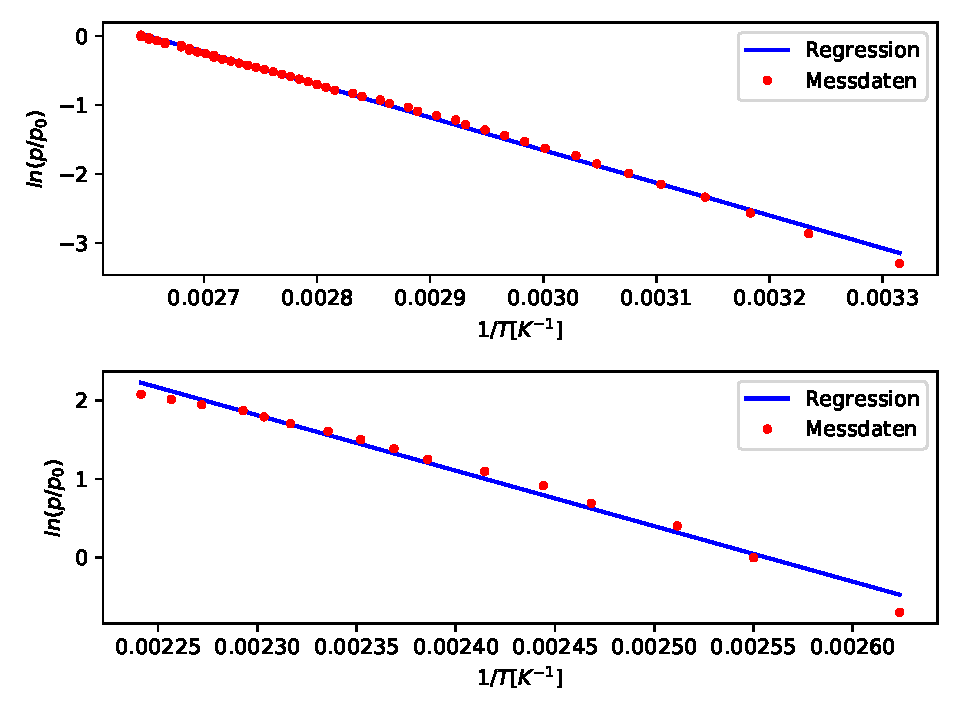
\includegraphics[scale = 0.75]{Auswertung/a.pdf}
  \caption{Dampfdruckkurve des Wassers}
  \label{fig:Dampfdruckkurve}
\end{figure}
Die eingezeichneten Regressionen haben nun Funktionsgleichungen der Form von Gleichung \eqref{eqn:dampfdruck2} mit
\begin{align*}
  \frac{L}{R} &= \SI{4738.75 \pm 34.25}{\kelvin} \\
  c           &= \num{12.56 \pm 0.0973} 
\end{align*}
für die Messwerte bei niedrigem und
\begin{align*}
  \frac{L}{R} &=  \SI{7054.89 \pm 226.93}{\kelvin}\\
  c           & =\num{18.03 \pm 0.54}
\end{align*}
bei hohem Druck. Die Unsicherheit der Parameter wurden genau wie die Regression mit \textit{nummeric python} 
berechnet.
\\
Die Steigung der Gerade ist demnach
\begin{equation}
  m=-\frac{L}{R} \Leftrightarrow L=-m\cdot R. \label{eqn:L}
\end{equation}

\subsection{Die Verdampfungswärme}
Mit Gleichung \eqref{eqn:L} kann nun die gemittelte Verdampfungswärme des Wassers berechnet werden.
Durch Einsetzen folgt für die Messwerte aus Tabelle \ref{tab:niedringe}
\begin{equation*}
  L=\SI{39400.195\pm284.792}{\joule\per\mole}.
\end{equation*}
Die Unsicherheit folgt wieder aus der von \textit{nummeric python} berechneten Unsicherheit der Parameter.
\\
Die äußere Verdampfungswärme $L_a$ ist die Energie, die benötigt wird, um das Volumen des Wassers von
$V_F$ auf $V_D$ zu vergößern. Demnach gilt für $L_a$ nach der idealen Gasgleichung
\begin{equation*}
  L_a=pV=RT.
\end{equation*}
Eine Abschätzung mit $T=\SI{373}{kelvin}$ ergibt
\begin{equation*}
  L_a=\SI{3101.29}{\joule\per\mole}.
\end{equation*}
Die Differenz der gemittelten Verdampfungswärme $L$ und der äußeren Verdampfungswärme $L_a$ ist dann 
die Energie $L_i$, die ein Wassermolekül besitzen muss, um die Anziehungskräfte der anderen Moleküle zu überwinden
und zu verdampfen. Bilden der Differenz liefert
\begin{equation*}
  L_i=L-L_a=\SI{0.376 \pm 0.003}{\electronvolt}.
\end{equation*}

\subsection{Abhängigkeit der Verdampfungswärme von der Temperatur}
Um die Verdampfungswärme $L$ in Abhängigkeit und der Termperatur zu bestimmen, formt man die
Clausius-Clapeyronsche Gleichung \eqref{eqn:clausiusclapeyron} nach L um und erhält
\begin{equation}
  L=T(V_D-V_F)\frac{dp}{dT}. \label{eqn:Clausius2}
\end{equation}
$V_F$ kann dabei gegenüber $V_D$ vernachlässigt werden. $V_D$ kann zudem nicht mehr durch die
ideale Gasgleichung \eqref{eqn:gasgleichung} berechnet werden. Eine bessere Näherung für $V_D$
ist stattdessen 
\begin{align}
  &RT=\left(p+\frac{a}{V_D^2}\right) \qquad mit \quad a=\SI{0.9}{\joule\cubic\metre\per\square\mole}\\
  \Leftrightarrow \quad &V_D=\frac{RT}{2p}\pm\sqrt{\frac{R^2T^2}{4p^2}-\frac{a}{p}}. \label{eqn:Vd}
\end{align}
Durch Einsetzen in Gleichung \eqref{eqn:Clausius2} ergibt sich
\begin{equation}
  L=T\left(\frac{RT}{2p}\pm\sqrt{\frac{R^2T^2}{4p^2}-\frac{a}{p}}\right)\frac{dp}{dT}. \label{eqn:Clausius3}
\end{equation}
Um den Differentialquotienten $dp/dT$ zu bestimmen, wird ein Ausgleichspolynom dritten Grades
aus den Messwerten aus Tabelle \ref{tab:hohe} gebildet und dann abgeleitet. In Abbildung
\ref{fig:Polynom} wurde dieses Polynom mit Pythongraphisch dargestellt.
\begin{figure}
  \centering
  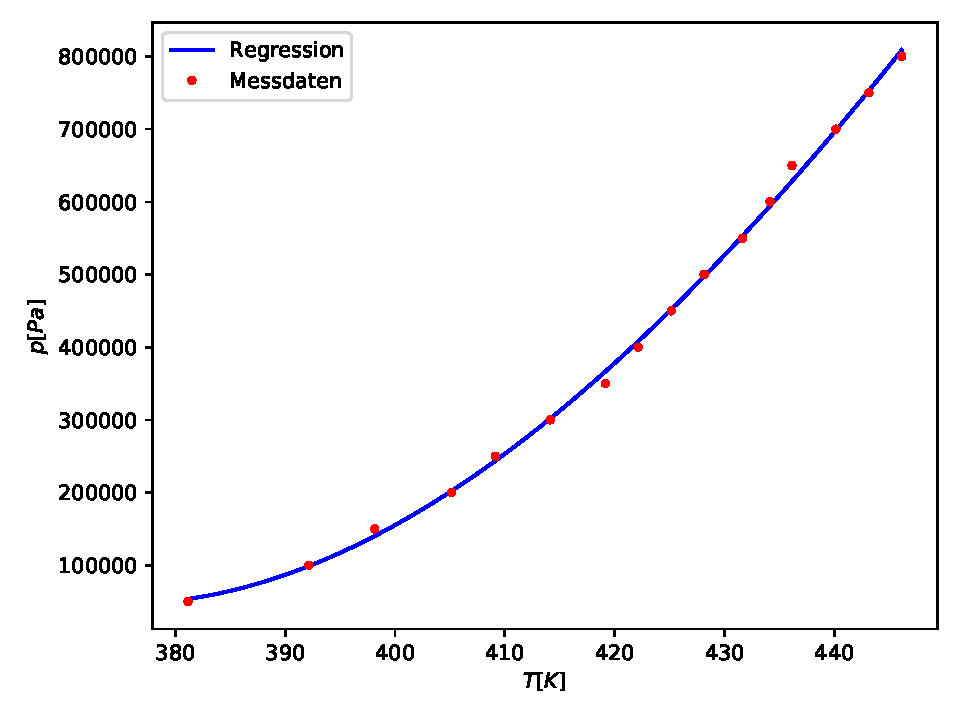
\includegraphics[scale = 0.75]{Auswertung/d1.pdf}
  \caption{Ein T-p-Diagramm mit Ausgleichspolynom}
  \label{fig:Polynom}
\end{figure}
Das Polynom hat dabei die Form
\begin{equation*}
  p=aT^3+bT^2+cT+d
\end{equation*}
\begin{align*}
  mit \quad a &= \SI{-0.5015\pm0.3859}{\pascal\per\cubic\kelvin}\\
      b &= \SI{750.50\pm479.79}{\pascal\square\kelvin}\\
      c &= \SI{-351292.70\pm198606.23}{\pascal\kelvin}\\
      d &= \SI{52690170.95\pm27370895.05}{\pascal}
\end{align*}
mit der Ableitung
\begin{equation*}
  \frac{dp}{dT}=3aT^2+2bT+c.
\end{equation*}
Auch hier wurden die Unsicherheiten mittels \textit{numpy} berechnet. Mit Gleichung 
\ref{eqn:Clausius3} kann nun $L(T)$ für die Messwerte aus Tabelle \ref{tab:hohe}
berechnet werden. Mittels Python wurden die Ergebnisse aus Tabelle \ref{tab:L} in Abbildung
\ref{fig:L} in einem T-L-Koordinatensystem dargestellt.
Dabei existieren nach Gleichung \ref{eqn:Vd} zwei Lösungen $L_1$ und $L_2$. $L_1$ ist dabei
die Lösung für den positiven und $L_2$ die Lösung für die negativen Wurzelterm.
\begin{table}
  \centering
      \caption{L in Abhängigkeit von T bei p<1bar}
      \label{tab:L}
      \sisetup{table-format=5.2}
      \begin{tabular}{S S S}
        \toprule
        {$T / \si{\kelvin}$} & {$ L1 \cdot \si{\mole\per\joule}$} & {$ L2 \cdot \si{\mole\per\joule}$} \\
        \midrule
        381.15 &   53692.43 &     242.76 \\
        392.15 &   75364.64 &     649.06 \\
        398.15 &   67826.04 &     856.78 \\
        405.15 &   66219.19 &    1085.11 \\
        409.15 &   59842.89 &    1211.06 \\
        414.15 &   57002.17 &    1360.70 \\
        419.15 &   54896.48 &    1502.82 \\
        422.15 &   51084.88 &    1586.96 \\
        425.15 &   48084.48 &    1668.54 \\
        428.15 &   45649.91 &    1747.52 \\
        431.65 &   44004.85 &    1835.11 \\
        434.15 &   41905.56 &    1897.51 \\
        436.15 &   39791.49 &    1947.66 \\
        440.15 &   39115.31 &    2036.59 \\
        443.15 &   37955.11 &    2101.95 \\
        446.15 &   36910.54 &    2164.46 \\
        \bottomrule
      \end{tabular}
    \end{table}
\begin{figure}
  \centering
  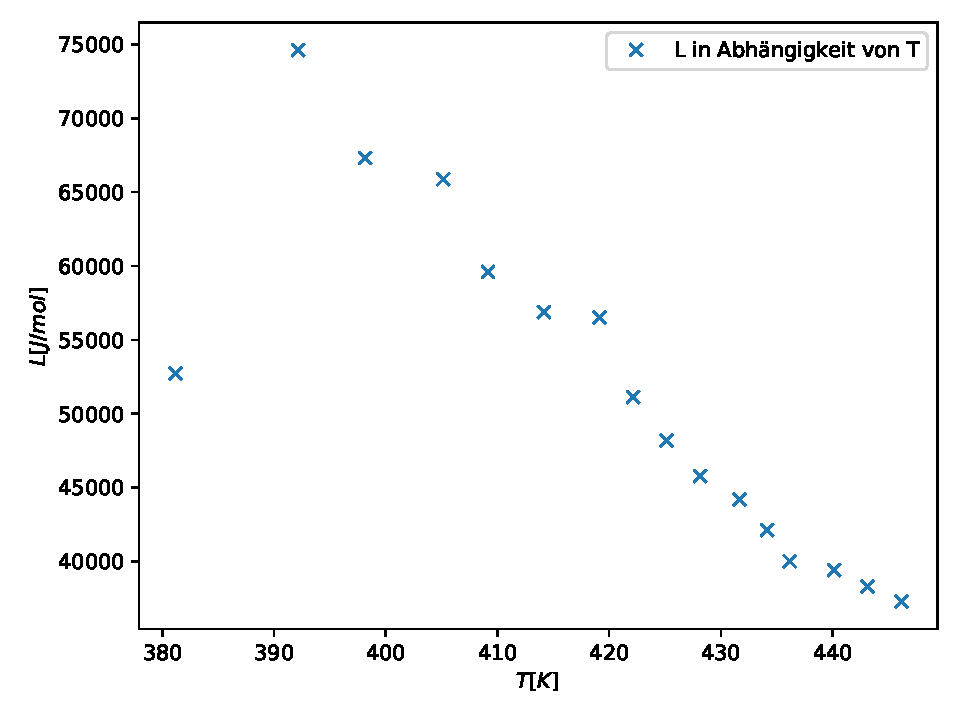
\includegraphics[scale = 0.75]{Auswertung/d2.pdf}
  \caption{L in Abhängigkeit von T}
  \label{fig:L}
\end{figure}
